\chapter{Listbox View}
\label{sec:listbox_view}
A Listbox View displays the DBObject data as text in tables, to allow textual data inspection. When started, it presents itself in the following manner.

\begin{figure}[H]
    \hspace*{-2cm}
    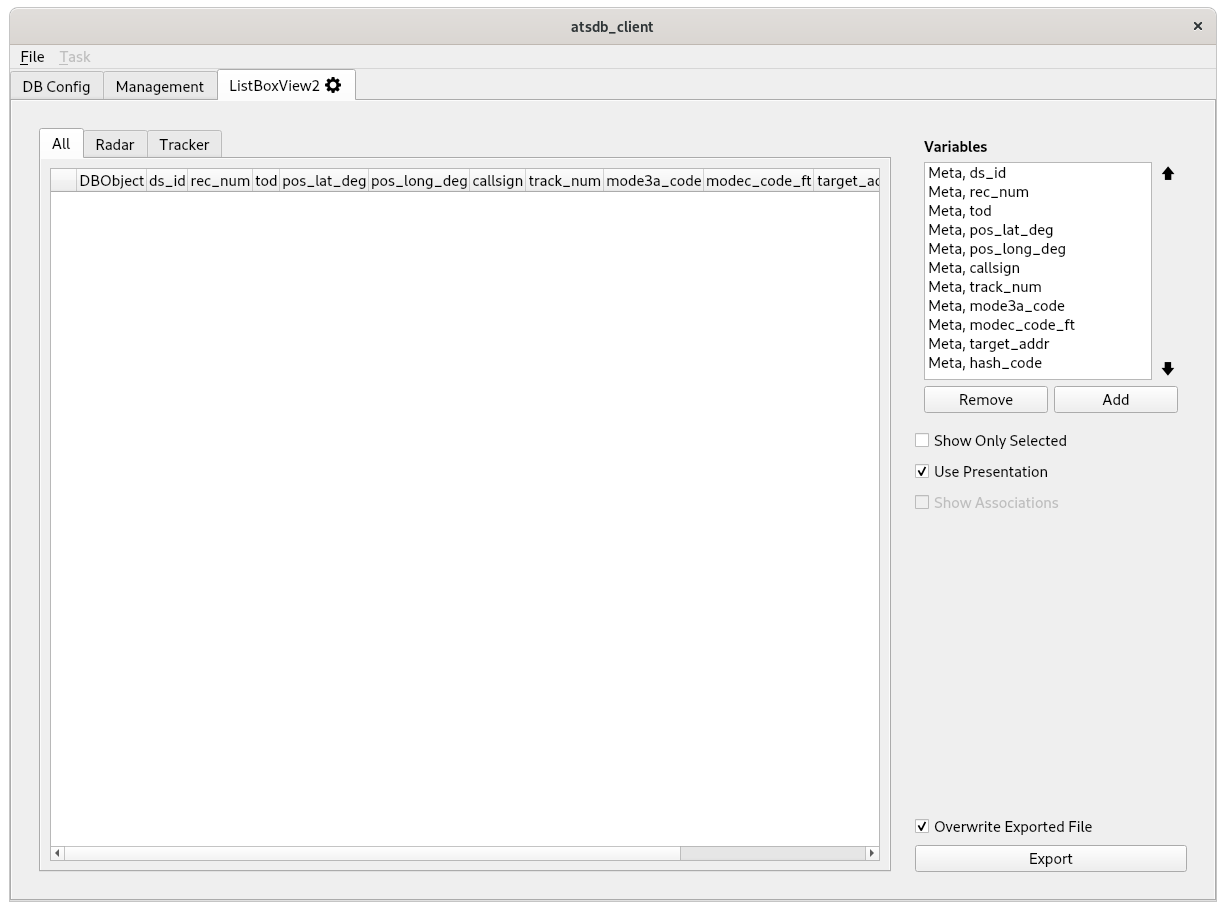
\includegraphics[width=18cm,frame]{../screenshots/listbox_start.png}
  \caption{Listbox View startup}
  \label{fig:listbox_start}
\end{figure}

\section{Layout}


On the left side, a number of tabs exist as 'All' and for each active DBO, each of which contains a table. \\

On the right side, a configuration area exists which allows configuration of what data is loaded and how it is displayed. \\

Both areas can be resized and hidden if wanted.

\section{Data Loading}

To load the data use the the mechanism described in Section \nameref{sec:management_dbos} can be used. To filter the dataset, the mechanism described in Section \nameref{sec:filtering} can be used. \\

\begin{figure}[H]
    \hspace*{-2cm}
    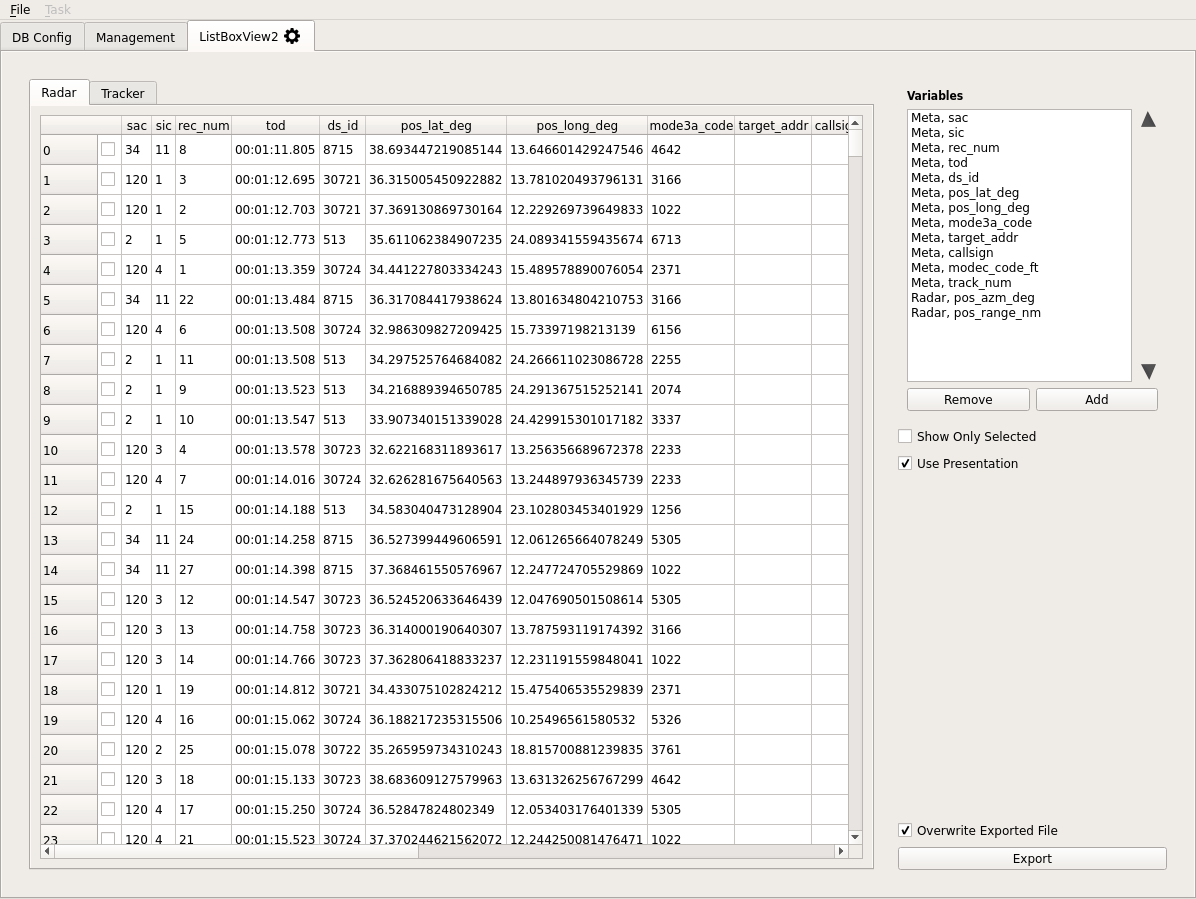
\includegraphics[width=18cm,frame]{../screenshots/listbox_loaded.png}
  \caption{Listbox View after loading}
\end{figure}

Once updated, the tables are filled with text representing the values of the DBObject variables.  If a value is undefined its cell is empy. For each DBO, a dedicated table is shown, as well as the 'All' table, where data from all DBOs are collectively shown. \\

Please \textbf{note} that since some variable might only exist in some DBObjects, the number of columns for different DBObjects may differ. \\

\section{Usage}

\subsection{Selection}
In the first column in the tables, checkboxes are shown, indicating whether that target report is currently selected. Selection may be changed by selecting/de-selecting the respective checkboxes or in other views (cross-selection). If the selection is changed in one of the other views, this view is updated automatically.


\subsection{Variable List}
All DBO variables which are loaded from the database are shown in the 'Variables' list. This list is ordered, and like all configuration elements persistent. Ordering can be changed by selecting (clicking on) a variable and using the up/down buttons. \\

When pressing the 'Remove' button, a selected variable is removed.  Pressing the 'Add' button allows appending a variable to the list using a context-menu. \\

If Meta variables are used, they are display in all DObjects they exist. If DBObject variable is used, it is only displayed in it's native object.

\begin{figure}[H]
    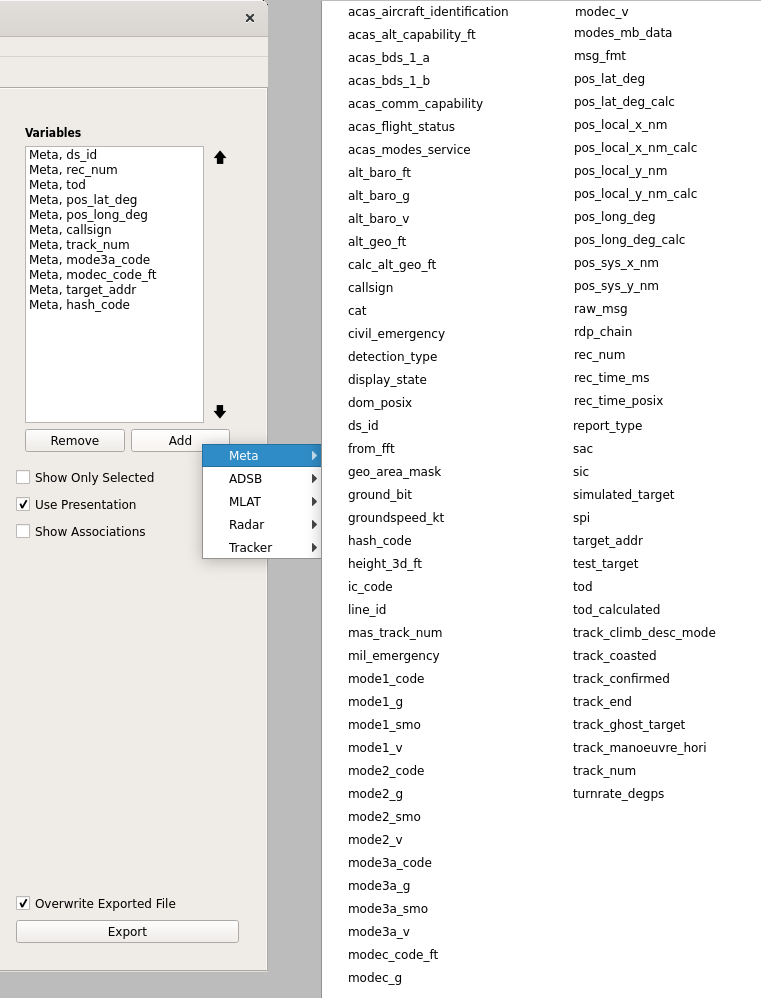
\includegraphics[width=16cm,frame]{../screenshots/listbox_add.png}
  \caption{Listbox View adding of variables}
\end{figure}


\subsection{Show Only Selected}
When this checkbox is checked, only target reports selected in other views are shown. If this is active, de-selecting a target report removes it from the shown data.

\subsection{Use Presentation}
When this checkbox is checked, the so called presentation mode is used. In the database, the variables might have different units or a data representation which is not easy to read. For this purpose, a presentation mode was introduced to e.g. show a Mode A code as octal, or a Time of Day not in seconds since midnight but in HH::MM:SS.SS format. \\

When the 'Use Presentation' checkbox is not checked, the original database values are presented (and exported).

\subsection{Show Associations}
When this checkbox is checked, the associated UTNs are shown for each target report. If no UTN is shown, this target reports was never associated to an UTN, if several are shown (e.g. '1,2,4') this target report was used in several UTNs. \\

This checkbox can only be used if association information is present in the database.

\begin{figure}[H]
    \hspace*{-2cm}
    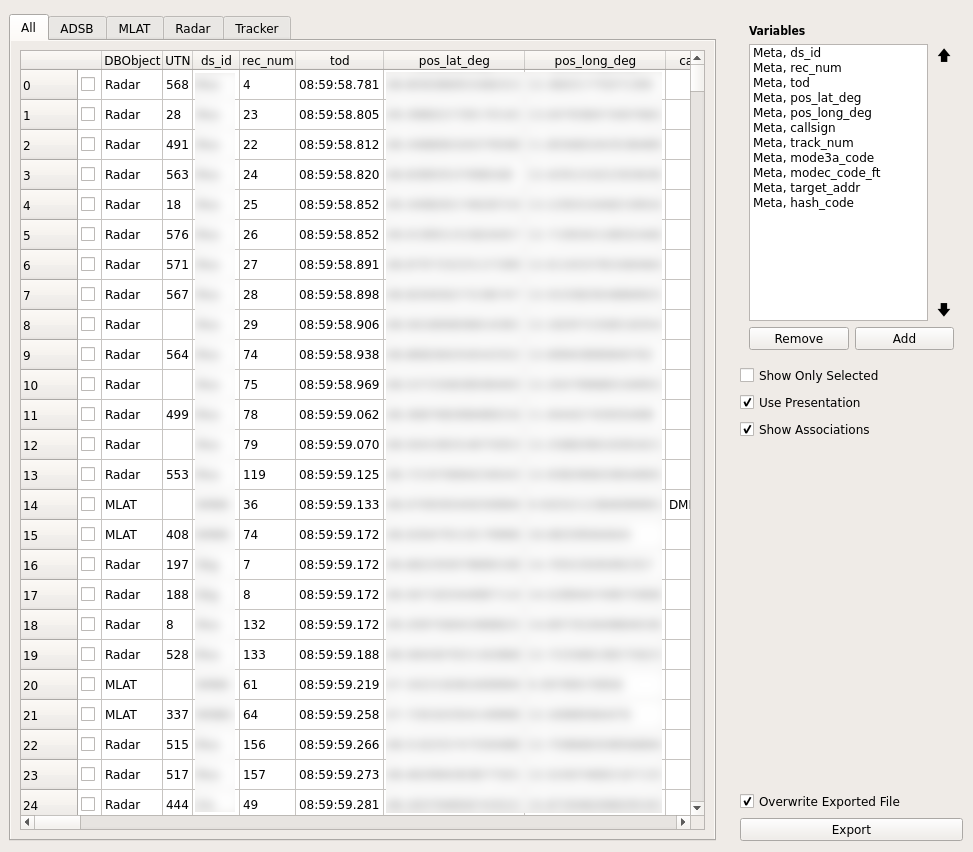
\includegraphics[width=18cm,frame]{../screenshots/listbox_loaded_assoc.png}
  \caption{Listbox View after loading with associated UTNs}
\end{figure}


\subsection{Exporting}
\label{sec:exporting}

The data from the current DBO table can be exported to a comma-separated value (CSV) text file. \\

For this example a Mode 3/A code filter was used to load only target reports and system track updates from a single target. \\

When pressing the 'Export' button, a dialog is opened.

\begin{figure}[H]
    \hspace*{-2cm}
    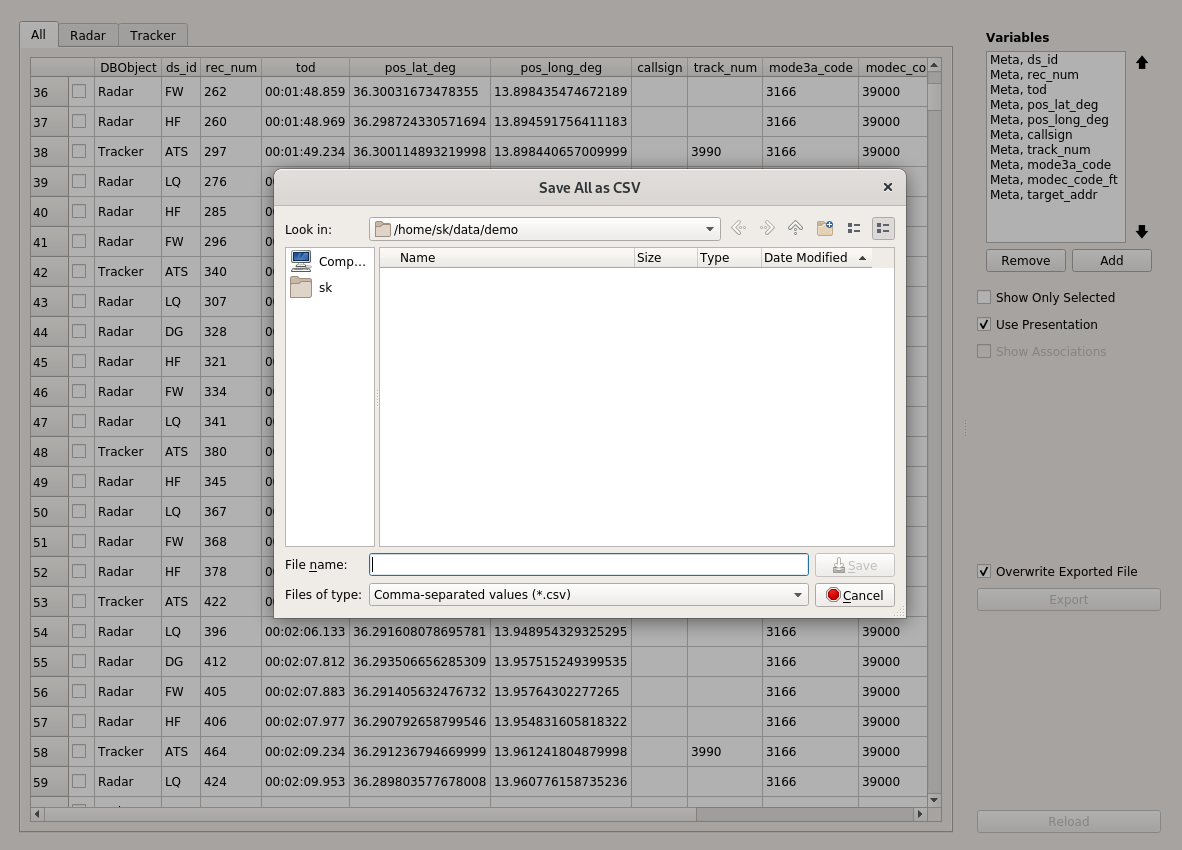
\includegraphics[width=18cm,frame]{../screenshots/listbox_export.png}
  \caption{Listbox View export}
\end{figure}

Choose a filename, and press 'Save' to save the data. If the 'Overwrite Exported File' checkbox was checked, an existing file is automatically overwritten. Please \textbf{note} that exporting might take some time for larger datasets, and currently no status indication is given.\\

After export, a dialog is shown indicating that the export was completed.

\begin{figure}[H]
  \center
    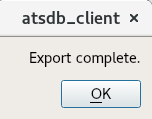
\includegraphics[width=18cm,frame]{../screenshots/listbox_exported.png}
  \caption{Listbox View export done}
\end{figure}

The exported file can be opened in any editor, or for example imported into LibreOffice Calc.

\begin{figure}[H]
    \hspace*{-2.5cm}
    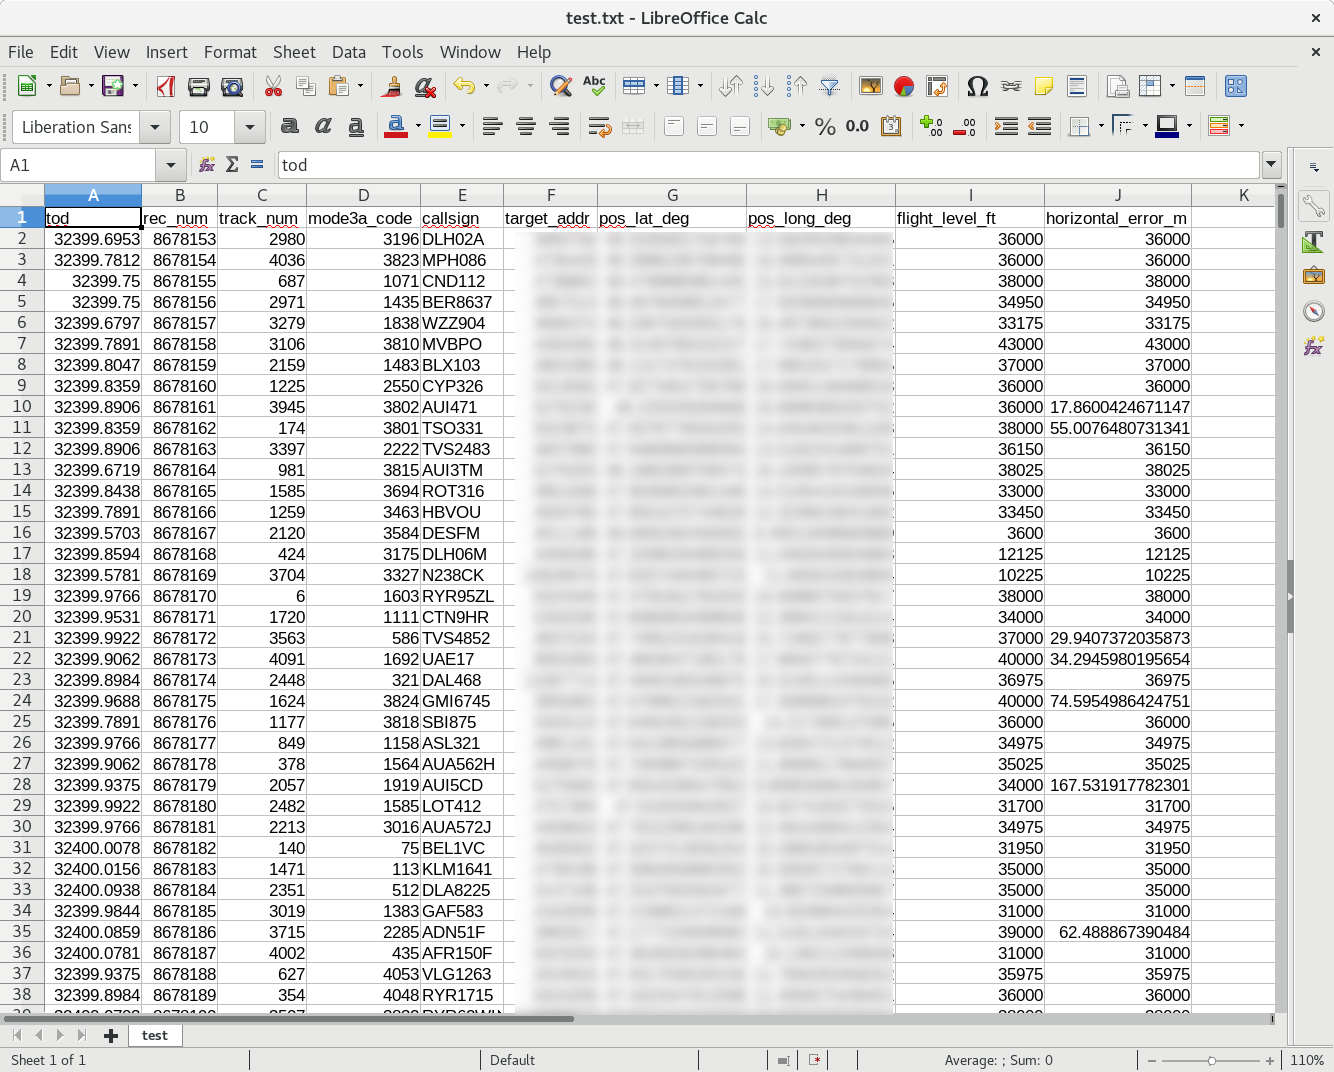
\includegraphics[width=19cm]{../screenshots/listbox_exported_calc.png}
  \caption{Listbox View export in LibreOffice Calc}
\end{figure}
 
\subsection{Reload}

Additionally, if a change is made that requires re-loading of the data (e.g. additional data should be displayed) the 'Reload' button becomes available, and can be used to trigger a loading process as in Section \nameref{sec:management_dbos}. 
